\subsection{Question 1}
\begin{enumerate}
\item Le reseau représentant une sémaphore
\begin{figure}[H]
  \centering
  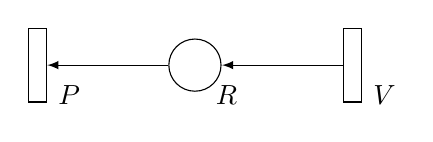
\begin{tikzpicture}
    % Liste des places
    \draw (0,0) node[below right = 4pt] {$R$};
    \node[draw,circle,scale=2] (R) at (0, 0) {};
    
      % Liste des transitions
    \draw (2,0) node[below right= 4pt] {$V$};
    \node[draw,rectangle,yscale=4] (V) at (2, 0) {};
    \draw (-2,0) node[below right= 4pt] {$P$};
    \node[draw,rectangle,yscale=4] (P) at (-2, 0) {};

     % Liste des arcs
    \draw[->,>=latex] (V) -- (R);
    \draw[->,>=latex] (R) -- (P);

  \end{tikzpicture}
  \caption{Réseau de petri associé à la sémaphore} \label{fig:M1}
\end{figure}


\item Simulation de l'évolution du réseau
Lorsqu'une ressource est mise à disposition, on a :

\begin{figure}[H]
  \centering
  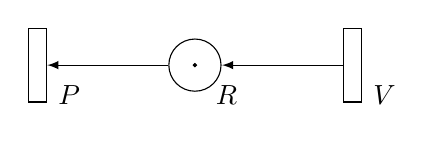
\begin{tikzpicture}
    % Liste des places
    \draw (0,0) node[below right = 4pt] {$R$};
    \node[draw,circle,scale=2] (R) at (0, 0) {};
    
      % Liste des transitions
    \draw (2,0) node[below right= 4pt] {$V$};
    \node[draw,rectangle,yscale=4] (V) at (2, 0) {};
    \draw (-2,0) node[below right= 4pt] {$P$};
    \node[draw,rectangle,yscale=4] (P) at (-2, 0) {};

     % Liste des arcs
    \draw[->,>=latex] (V) -- (R);
    \draw[->,>=latex] (R) -- (P);

     %Marquage
    \draw [fill](0,0) circle (0.02);

  \end{tikzpicture}
  \caption{Réseau de petri associé à la sémaphore} \label{fig:M1}
\end{figure}

On met à disposition une nouvelle ressource: 

\begin{figure}[H]
  \centering
  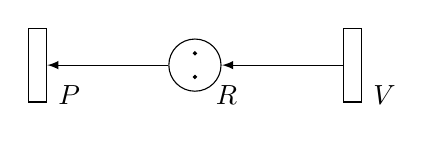
\begin{tikzpicture}
    % Liste des places
    \draw (0,0) node[below right = 4pt] {$R$};
    \node[draw,circle,scale=2] (R) at (0, 0) {};
    
      % Liste des transitions
    \draw (2,0) node[below right= 4pt] {$V$};
    \node[draw,rectangle,yscale=4] (V) at (2, 0) {};
    \draw (-2,0) node[below right= 4pt] {$P$};
    \node[draw,rectangle,yscale=4] (P) at (-2, 0) {};

     % Liste des arcs
    \draw[->,>=latex] (V) -- (R);
    \draw[->,>=latex] (R) -- (P);

     %Marquage
    \draw [fill](0,0.15) circle (0.02);
    \draw [fill](0,-0.15) circle (0.02);

  \end{tikzpicture}
  \caption{Réseau de petri associé à la sémaphore} \label{fig:M1}
\end{figure}

Une ressource est monopolisée, on revient à la fig. 20\\
Et si on monopolise une nouvelle ressource on revient au graphe initial (fig. 19)\\
A ce moment, il est impossible d'acceder à une ressource tant qu'elle n'est pas mise à disposition comme vu précédemment.

\item Transitions concurente?

Dans le cas où le marquage de la place $R$ est non nul, les deux transitions peuvent être franchit indépendement.
Dans le cas ou le marquage de la place $R$ est nul, la transition $V$ peut être franchit, mais pas la transition $P$.
Cependant, l'incapacité de franchissement de P n'est pas du au franchissement de V.
Donc ces deux transition ne sont pas concurrentes entre elles.

Toutefois, les transitions $P$ et $V$ peuvent être concurrentes avec elles-mêmes.



\end{enumerate}

\subsection{Question 2}
\begin{enumerate}
\item Le reseau coloré représentant une sémaphore

\begin{figure}[H]
  \centering
  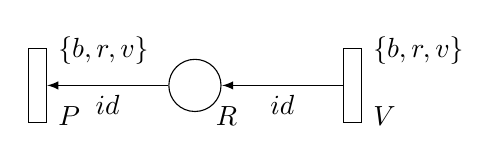
\begin{tikzpicture}
    % Liste des places
    \draw (0,0) node[below right = 4pt] {$R$};
    \node[draw,circle,scale=2] (R) at (0, 0) {};
    
      % Liste des transitions
    \draw (2,0) node[below right= 4pt] {$V$};
    \draw (2,0) node[above right= 4pt] {$\{b,r,v\}$};
    \node[draw,rectangle,yscale=4] (V) at (2, 0) {};
    \draw (-2,0) node[below right= 4pt] {$P$};
    \draw (-2,0) node[above right= 4pt] {$\{b,r,v\}$};
    \node[draw,rectangle,yscale=4] (P) at (-2, 0) {};

     % Liste des arcs
    \draw[->,>=latex] (V) -- (R)node[midway, below]{$id$};
    \draw[->,>=latex] (R) -- (P)node[midway, below]{$id$};

  \end{tikzpicture}
  \caption{Réseau de petri associé à la sémaphore} \label{fig:M1}
\end{figure}

Ici, grâce aux couleurs, on peut représenter les différents processus (ici noté $r,v,b$) qui vont pouvoir accéder à une ressource donnée.

\item Simulation de l'évolution du réseau
  Lorsque l'on met une ressource à disposition, on peut choisir quel type de processus va pouvoir y accéder :\\

\begin{figure}[H]
  \centering
  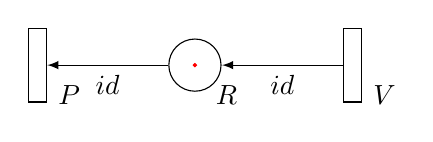
\begin{tikzpicture}
    % Liste des places
    \draw (0,0) node[below right = 4pt] {$R$};
    \node[draw,circle,scale=2] (R) at (0, 0) {};
    
      % Liste des transitions
    \draw (2,0) node[below right= 4pt] {$V$};
    \node[draw,rectangle,yscale=4] (V) at (2, 0) {};
    \draw (-2,0) node[below right= 4pt] {$P$};
    \node[draw,rectangle,yscale=4] (P) at (-2, 0) {};

     % Liste des arcs
    \draw[->,>=latex] (V) -- (R)node[midway, below]{$id$};
    \draw[->,>=latex] (R) -- (P)node[midway, below]{$id$};

     %Marquage
    \draw [fill, red](0,0) circle (0.02);

  \end{tikzpicture}
  \caption{Sémaphore avec une ressource rouge disponible} \label{fig:M1}
\end{figure}

Ici seul un processus ``rouge'' peut accéder à la ressource.\\
On met à disposition une ressource verte cette fois: 

\begin{figure}[H]
  \centering
  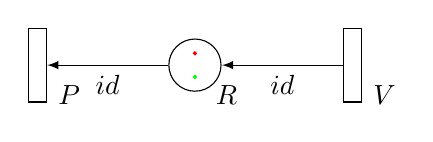
\begin{tikzpicture}
    % Liste des places
    \draw (0,0) node[below right = 4pt] {$R$};
    \node[draw,circle,scale=2] (R) at (0, 0) {};
    
      % Liste des transitions
    \draw (2,0) node[below right= 4pt] {$V$};
    \node[draw,rectangle,yscale=4] (V) at (2, 0) {};
    \draw (-2,0) node[below right= 4pt] {$P$};
    \node[draw,rectangle,yscale=4] (P) at (-2, 0) {};

     % Liste des arcs
    \draw[->,>=latex] (V) -- (R)node[midway, below]{$id$};
    \draw[->,>=latex] (R) -- (P)node[midway, below]{$id$};

     %Marquage
    \draw [fill, red](0,0.15) circle (0.02);
    \draw [fill, green](0,-0.15) circle (0.02);

  \end{tikzpicture}
  \caption{Sémaphore avec deux ressources différentes} \label{fig:M1}
\end{figure}

\item Transitions concurente?

Pour les même raison que dans le reseau non coloré, les transitions $P$ et $V$ ne sont pas concurrentes entre elles mais peuvent l'être avec elles-même.
\end{enumerate}
